\chapter*{Introduction}
\addcontentsline{toc}{chapter}{Introduction}
The triumph of the 20th century particle physics was the development of the Standard Model. Experiments determined the particle constituents of ordinary matter, and identified four forces binding matter and transforming it from one form to another. This success leads particle physicist to address even more fundamental questions, and explore deeper mysteries in science.\par
The Standard Model includes a third component beyond particles and forces, the Higgs mechanism. The Higgs mechanism permeates the universe, giving mass to the particles, and breaking the electro-weak force in two, the electromagnetic and the weak forces.\par
\begin{figure}[!hbt]
\centering
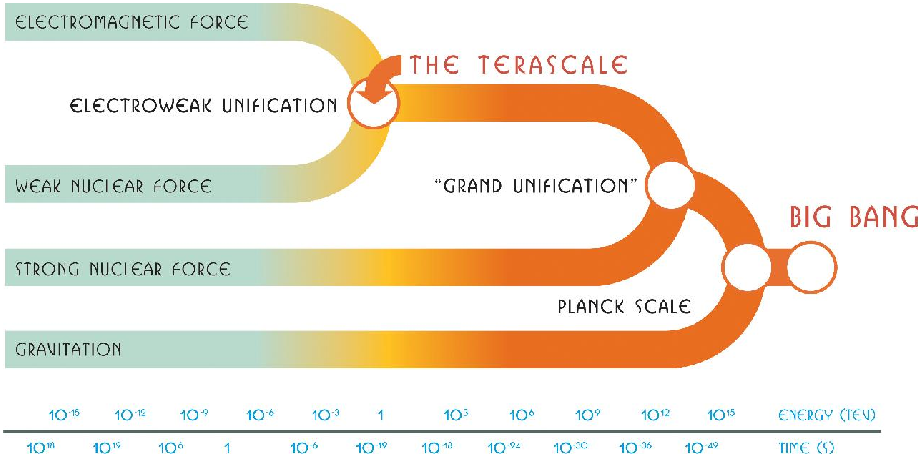
\includegraphics[scale=0.8,angle=0]{energyforce.pdf}\caption{The electromagnetic and electro-weak forces unify at the Terascale.}\label{f:energyforce}
\end{figure}
Experiments in the Terascale could test the idea that fundamental forces originate from a single unified force, see Fig. \ref{f:energyforce}, and search for evidence of a related unified origin of matter involving supersymmetry. They could distinguish among patterns of phenomena to judge different unification models, providing a telescopic view of the ultimate unification.\par
% \section*{The exploration of high energy physics}
% \addcontentsline{toc}{section}{The exploration of high energy physics}
There are two ways to explore the subatomic world, the first is to go to higher energy to discover new particles and measure their properties, the second is to increase the precision of the measurements to detect rare processes and make detailed studies.\par
The LHC allows the exploration of the electroweak symmetry breaking mechanism and other physical phenomena at the TeV scale, like the CP violation problem, the quark gluon plasma at the search of new physics beyond the Standard Model such as supersymmetry (SUSY) among others. The future linear collider beam energy will be determined by the LHC discoveries.\par
\textbf{Higgs searches:} The 4th of July of 2012, in a seminar held at CERN, the collaborations of the Experiments CMS and ATLAS presented an update of the Higgs of the Higgs searches status. At a confidence level of 4.9$\sigma$ for CMS \cite{TheCMSCollaboration21122012}, and 5.1$\sigma$ for ATLAS \cite{TheATLASCollaboration21122012} from the Higgsless Standard Model, signals of a boson with a mass around $m_h=125$~GeV were found with a strong spin-0 indication and coupling parameters consistent with the properties of the Standard Model Higgs Particle. First results on various rare production decay modes have been obtained but more data is needed to observe these models. Many analyses are ongoing and more updates are constantly presented.\par
\textbf{Heavy Flavour and CP Violation:} The experiments of the LHC, led by the LHCb, have carried out several important findings and measurements in the heavy flavour sector. New previously unobserved states have been observed for the very first time during the last years like the states $X_b$, $\Xi_a$ and $\Lambda_s^0$. Also the measurement of the quantum numbers of the states $X(3872)$ with $J^{PC}=1^{++}$, have been determined to the 8$\sigma$ level. The CP violation of the oscillation in D and B mesons have been measured to the 9.1$\sigma$ confidence level discovering the same violation in $B_s$ systems. The CP angle $\gamma$ is known with a precision without precedents ($\gamma=(67\pm12)$\textdegree). Finally, some very rare decays like $B_s\rightarrow\mu^+\mu^-$, $B^0\rightarrow K^*\mu^+\mu^-$ and $D_s^+\rightarrow\pi^+\mu^+\mu^-$ have been observed, with possible implications on the analysis of new physics.\par
\textbf{Quark-gluon Plasma:} The quark-gluon plasma is produced in ultra-relativistic heavy ion collisions. The conditions observed at the LHC experiments (ALICE, ATLAS and CMS) are in agreement with the observations carried out at RHIC. It has been confirmed that the hydrodynamics model helps in the understanding of the behaviour of the processes occurred during the collision. It is still far from being completely understood.\par
\textbf{SUSY and Dark Matter searches:} One of the problem that arises is the stabilization of the Higgs mass and its divergence when quantum divergence is considered. The solution involves a new principle of nature called supersymmetry (SUSY), a new symmetry that unifies bosons and fermions. After data collected during 2011 and 2012, SUSY searches at the LHC did not find any evidence of any light superpartner (squark or gluino) and it has pushed their mass limits beyond 1~TeV with the constrained model~\cite{Kraml:2012er}.\par
\vspace*{0.6cm}
The Second run of the LHC at 13~TeV will provide more information about the physics at high energies.\par

\section*{Circular or linear colliders}
\addcontentsline{toc}{section}{Circular or linear colliders}
Higher energies have been usually explored with hadron colliders and the precision measurements has been done afterwards by lepton colliders, however, lepton circular colliders are limited by radiation. When particles traverse magnetic fields they emmit photons and this photons make the beam loose energy per turn given by
\begin{equation}
 \Delta E_{turn}=\frac{E^4}{3\rho m_0^4c^8}
\end{equation}
where $m_0$ is the rest mass of the particle, $c$ is the speed of light, $\rho$ is the curvature radius to the trajectory produced by the magnet and $E$ is the beam energy. The highest energy lepton collision, 209~GeV, have been reached with electron and positron coliding beams in LEP at CERN.  In spite of the 27~km circumference of LEP the beam energy was limited by synchrotron radiation losses, just compensated by a powerfull superconducting RF system providing up to 3640~MV per revolution \cite{Assmann:549223}.\par
% \section{Purpose of a linear collider}
